\documentclass[a4paper,11pt]{article}

\usepackage[finnish]{babel}
\usepackage[utf8]{inputenc}
\usepackage[margin=2cm]{geometry}
\usepackage{amsfonts,amsmath,amssymb,amsthm,enumitem}
\usepackage{microtype}
\usepackage{booktabs}
\usepackage{pgf}
\usepackage{tikz}
\usepackage{tikz-qtree}
\usetikzlibrary{arrows,automata}

\setenumerate{listparindent=\parindent}

\newtheorem*{claim}{Väite}

\newcommand{\set}[1]{{\left\{ #1 \right\}}}
\newcommand{\ceil}[1]{{\left\lceil#1\right\rceil}}
\newcommand{\Nat}{\mathbb{N}}
\newcommand{\ve}{\varepsilon}

\newenvironment{automata}[1][2.8]%
{\begin{tikzpicture}[->,>=stealth',shorten >=1pt,auto,node distance=#1cm,semithick]}%
{\end{tikzpicture}}

\newenvironment{centerautomata}[1][2.2]%
{\begin{center}\begin{automata}[#1]}%
{\end{automata} \end{center}}

\begin{document}

\subsection*{582206 Laskennan mallit, syksy 2012 \\
  \textmd{7. harjoitusten malliratkaisut \\
    Juhana Laurinharju ja Jani Rahkola}}

\begin{enumerate}
  \item
    Esitä pinoautomaatti seuraaville kielille.
    \begin{enumerate}
      \item
        Kaikki palindromit aakkostosta $\Sigma = \set{a, b, c}$.

        \begin{automata}
            \node[initial, state] (q0) {$q_0$};
            \node[state] (q1) [right of=q0] {$q_1$};
            \node[state] (q2) [right of=q1] {$q_2$};
            \node[state, accepting] (q3) [right of=q2] {$q_3$};

            \path
            (q0) edge node {$\ve, \ve \to \$ $} (q1)
            (q1) edge [loop below] node {$\begin{aligned}
                              a, \ve \to a \\
                              b, \ve \to b \\
                              c, \ve \to c
                            \end{aligned}$} (q0)
            (q1) edge node {$\begin{aligned}
                                \ve, \ve \to \ve\\
                                a, \ve \to \ve \\
                                b, \ve \to \ve \\
                                c, \ve \to \ve
                            \end{aligned}$} (q2)
            (q2) edge [loop below] node {$\begin{aligned}
                                a, a \to \ve \\
                                b, b \to \ve \\
                                c, c \to \ve
                            \end{aligned}$} (q2)
            (q2) edge node {$\ve, \$ \to \ve$} (q3);

        \end{automata}

      \item
        $\set{a^ib^j \mid 0 \le i \le j}$ missä $\Sigma = \set{a, b, c}$

        \begin{automata}
            \node[initial, state] (q0) {$q_0$};
            \node[state] (q1) [right of=q0] {$q_1$};
            \node[state] (q2) [right of=q1] {$q_2$};
            \node[state] (q3) [right of=q2] {$q_3$};

            \path
            (q0) edge node {$\ve, \ve \to \$ $} (q1)
            (q1) edge [loop below] node {$a, \ve \to 1$} (q1)
            (q1) edge node {$\ve, \ve \to \ve$} (q2)
            (q2) edge [loop below] node {$b, 1 \to \ve$} (q2)
            (q2) edge node {$\ve, \$ \to \ve$} (q3)
            (q3) edge [loop below] node {$b, \ve \to \ve$} (q3);
        \end{automata}

      \item
        $\set{a^ib^jc^k \mid j = i + k}$ missä $\Sigma = \set{a, b, c}$

        \begin{automata}
            \node[initial, state] (q0) {$q_0$};
            \node[state] (q1) [above of=q0] {$q_1$};
            \node[state] (q2) [right of=q1] {$q_2$};
            \node[state] (q3) [right of=q2] {$q_3$};
            \node[state] (q4) [right of=q3] {$q_4$};
            \node[state, accepting] (q5) [below of=q4] {$q_5$};

            \path
            (q0) edge node {$\ve, \ve \to \$ $} (q1)
            (q1) edge [loop above] node {$a, \ve \to 1$} (q1)
            (q1) edge node {$\ve, \ve \to \ve$} (q2)
            (q2) edge [loop above] node {$b, 1 \to \ve$} (q2)
            (q2) edge node {$\ve, \$ \to \$ $} (q3)
            (q3) edge [loop above] node {$b, \ve \to 1$} (q3)
            (q3) edge node {$\ve, \ve \to \ve$} (q4)
            (q4) edge [loop above] node {$c, 1 \to \ve$} (q4)
            (q4) edge node {$\ve, \$ \to \ve$} (q5) ;
        \end{automata}

      \item
        Kaikki aakkoston $\Sigma = \set{0, 1}$ merkkijonot joissa nollia on
        kaksi kertaa niin paljon kuin ykkösiä.
    \end{enumerate}

  \item
    Tarkastellaan kielioppia
%
    \begin{align*}
      S & \to S+T \mid T \\
      T & \to T*F \mid F \\
      F & \to (S) \mid a
    \end{align*}
%
    Muodosta merkkijonon $s=( a+ a)* a$ jäsennyspuu tämän kieliopin
    mukaisesti.

    Etsi jäsennyspuusta jokin juuresta lehteen johtava polku, jolla sama
    muuttuja esiintyy kahdessa solmussa. Muodosta tämän perusteella
    toistuvuusominaisuuden todistuksen ideaa mukaillen jokin merkkijonon $s$
    jako osiin $s=uvxyz$, joilla merkkijono $uv^ixy^iz$ kuuluu tarkasteltavaan
    kieleen kaikilla $i\in N$.

    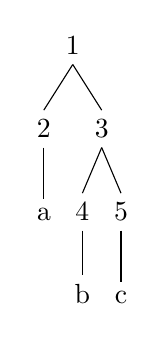
\begin{tikzpicture}
        {\Tree [.1 [.2 a ] [.3 [.4 b ] [.5 c ] ] ]}
    \end{tikzpicture}

  \item
    Olkoon $A$ aakkoston $\set{0,1}$ kieli, joka koostuu niistä
    merkkijonoista, joissa on sama määrä nollia ja ykkösiä. Tällä kielellä on
    kontekstiton kielioppi
%
    \begin{equation*}
      S \to SS \mid 0S1 \mid 1S0 \mid \ve
    \end{equation*}
%
    \begin{enumerate}
    \item
      Kielen $A$ eräs toistuvuuspituus on 4. Esitä kieleen $A$ kuuluvalle
      merkkijonolle $s=001101$ kaikki eri tavat jakaa se osiin $s=uvxyz$
      toistuvuusominaisuuden ehdot toteuttavalla tavalla (lause 2.30; Sipser
      Theorem 2.34; tässä siis $p=4$).

      \begin{tabular}{ccccc}
          \toprule
          $u$         & $v$  & $x$ & $y$  & $z$ \\
          \midrule
                      &      &     & 0011 & 01\\
                      &      & 0   & 01   & 101\\
                      & 0    &     & 011  & 01\\
                      & 0    & 0   & 1    & 101\\
                      & 0    & 01  & 1    & 01\\
                      & 00   &     & 11   & 01\\
                      & 001  &     & 1    & 01\\
                      & 0011 &     &      & 01\\
          0           &      &     & 01   & 101\\
          0           &      &     & 0110 & 1\\
          0           &      & 01  & 10   & 1\\
          0           & 0    &     & 1    & 101\\
          0           & 0    &     & 110  & 1\\
          0           & 0    & 1   & 1    & 01\\
          0           & 01   &     &      & 101\\
          0           & 01   &     & 10   & 1\\
          0           & 01   & 1   &      & 01\\
          0           & 01   & 10  &      & 1\\
          0           & 011  &     & 0    & 1\\
          0           & 0110 &     &      & 1\\
          00          &      & 1   & 10   & 1\\
          00          &      & 11  & 01   & \\
          00          & 1    & 1   & 0    & 1\\
          001         &      &     & 10   & 1\\
          001         &      & 1   & 01   & \\
          001         & 1    &     & 0    & 1\\
          001         & 10   &     &      & 1\\
          001         & 10   & 1   &      & \\
          0011        &      &     & 01   & \\
          0011        & 0    &     & 1    & \\
          0011        & 01   &     &      &
          \bottomrule
      \end{tabular}

      Yhteensä 31 ehdot täyttävää jakoa.

    \item
      Onko kielellä $A$ pienempiä toistuvuuspituuksia kuin 4? Perustele.
    \end{enumerate}

  \item
    \begin{enumerate}
      \item
        Koostukoon aakkoston $\set{a,b,c}$ kieli $A$ merkkijonoista, joissa on
        yhtä monta $a$-, $b$- ja $c$-merkkiä. Osoita, että $A$ ei ole
        yhteydetön.

      \item
        Osoita, että kieli $\set{0^n1^n0^n1^n \mid n \in \Nat}$ ei ole
        yhteydetön.
    \end{enumerate}

  \item
    Anna yhteydetön kielioppi, joka tuottaa kielen $\set{a^ib^jc^k \mid i = 2j
      \text{ tai } j = 2k}$. Muodosta apulauseen 2.21 mukaisesti kieliopistasi
    pinoautomaatti, joka tunnistaa saman kielen.

  \item
    Tee alla olevasta pinoautomaatista Apulauseen 2.27 mukaisesti kielioppi.

    \begin{centerautomata}
      \node[initial,state,accepting]   (q0)                     {$q_0$};
      \node[state]           (q1) [above right of=q0] {$q_1$};
      \node[state,accepting] (q3) [below right of=q0] {$q_3$};
      \node[state]           (q2) [above right of=q3] {$q_2$};

      \path (q0) edge              node {$\ve, \ve \to \$ $} (q1)
            (q1) edge [loop above] node {$\begin{aligned}
                                           0, & \ve \to  0 \\
                                           1, & \ve \to  1
                                         \end{aligned}$} ()
                 edge              node {$\ve,\ve\to\ve$} (q2)
            (q2) edge [loop right] node {$\begin{aligned}
                                          0, & 0 \to \ve \\
                                          1, & 1 \to \ve
                                          \end{aligned}$} ()
                 edge              node {$\ve,\$ \to \ve$} (q3);
    \end{centerautomata}

  \item
    \begin{enumerate}
    \item
      Osoita, että jos $A$ on yhteydetön ja $B$ säännöllinen kieli, niin
      $A\cap B$ on yhteydetön.

      \emph{Vihje:} muodosta pinoautomaatin ja äärellisen automaatin
      leikkausautomaatti samaan tapaan kuin Jyrkin luentojen lauseessa 1.1
      (luentomateriaalin sivut 48--50).

    \item
      Tiedetään, että kieli $L$ on yhteydetön ja $R$ säännöllinen. Voidaanko
      tästä päätellä, että $L-R$ on yhteydetön? Entä $R-L$? Perustele.
    \end{enumerate}
\end{enumerate}

\end{document}
